\subsection{Data Requirements}
intro... 

\subsubsection{Data Model}
The design level data requirements are represented through a E/R diagram:

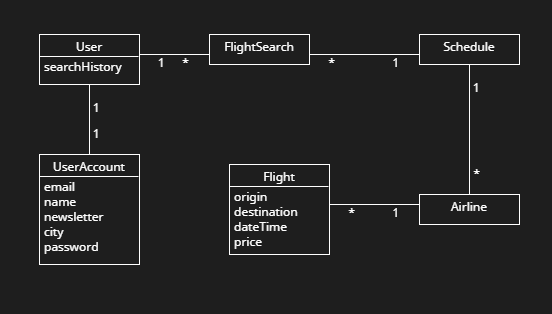
\includegraphics{resources/dataRelations.PNG}

\subsubsection{Data Dictionary}

DR2: Domain level data requirement

Class: User
The user is a Traveller or Travel Agency who has a user account in the product.

Examples:
1. A traveller who has a user account.
2. A travel agency who uses their user account to search flights.

Attributes:
email:      Text, 320 chars
            The user's email address. This email address is used for communication with the user outside the product.

name:       Text, 50 chars
            The name of the traveller or travel agency using the account.

newsletter: Boolean
            Wether the user wants mass email's from the product or not.

city:       Text, 35 chars
            The city the user's default origin is set to. This is the standard origin used when performing searches for the user.

\subsubsection{Virtual window}
Create a virtual window that shows the data that is to be displayed in the system. 

See this example 
# Traveller #374

## Personal Information

| Field     | Value                   |
|-----------|-------------------------|
| **Email** | exampleJohn@gmail.com   |
| **Name**  | John Doe                |
| **Utskick** | ● True  ○ False       |
| **City**  | New York                |

## Övervakningar (Monitoring)

| From | Price Max | To  |
|------|----------|-----|
| NY   | 3000 SEK | CPH |
| CPH  | 2500 SEK | NY  |
| ...  | ...      | ... |